\chapter{THE LHC AND THE CMS EXPERIMENT}\label{Ch2}

European Organisation for Nuclear Research, best know as CERN, is established in 1954 by 12 European countries and is based at the Franco-Swiss border in northwest Geneva, Switzerland. Today, the organisation operates the largest particle physics laboratory in the world and has 23 member states \cite{CERN:2771424} and many others that make up more than 11 thousand researches and more than 70 countries around the globe. CERN's main activity is to provide the particle accelerators and needed infrastructure for high energy physics research. The organisation hosts the LHC Experiment which is the world's largest particle collider.

This chapter introduces the structure and operations of the LHC and the CMS Detector on which the simulated Monte Carlo event samples are based in this thesis.

\section{The Large Hadron Collider}

The Large Hadron Collider consists of a 27-kilometre ring tunnel where the beams of particles (protons or lead ions) are accelerated with the help of superconducting magnets along with a number of accelerating systems. It was built between 1998 and 2008 and it lies 175 metres beneath the surface with a total cost of the project expected to be of the order of 4.4\$ billion. The initial design of the LHC aimed at the centre-of-mass energy of $\sqrt{s}=14$ TeV with a nominal peak luminosity of $\mathcal{L} = 10^{34}cm^{-2}s^{-1}$ \cite{Baconnier:257706}. The LHC collides proton-proton beams as well as lead-lead (Pb - Pb), proton-lead (p - PB) and Xenon-Xenon (Xe - Xe) nuclei to study heavy-ion collisions. The \textbf{\emph{LHC accelerator complex}} consist of a series of accelerators and is used to accelerate protons before being injected in the LHC, which will be explained shortly.

\subsection{Operation of the LHC}

The success of the LHC required two decade-long international collaboration. The initial studies started in the early 1980s when the The Large Electron Positron Collider (LEP) at CERN was not even running. CERN Council approved the construction of the LHC in 1994 and a technical design report was published the next year. Starting from 1998, the construction of the LHC was completed in 2008 and it succeeded to accelerate proton beams the same year \cite{lhcfirstbeams}. The first accelerated proton beams had an energy of 450 GeV per beam and later on the collisions at $\sqrt{s}=2.14$ TeV with respect to Tevatron at 1.96 TeV and made the LHC the highest-energy collider ever built. In 2010, LHC increased the beam energy to 3.5 TeV which was a world record of man-made particle acceleration.

Data collection started in 2010 and finished in 2013; this time period is known as Run I of the LHC. The CMS Experiment collected about 45$pb^{-1}$, 6 $fb^{-1}$ and 23 $fb^{-1}$ data at $\sqrt{s}=7$ TeV in 2010, 2011 and 2012, respectively. The data collected at Run I has lead the discovery of the Higgs boson. LHC entered an upgrade stage called Long Shutdown 1 (LS1) for two years when Run I is finished in 2012. LHC was upgraded in LS1 in the way of achieving its design performances, and started its operation again in 2015 for a period of 3 years known as Run II but his time the beam energy was 6.5 TeV. The Run II is finished in 2018 with a data amounting to about 150 $fb^{-1}$ and LHC entered LS2 with a schedule to be in Run III in 2022 at $\sqrt{s}=14$ TeV. The LS3 is planned to be the update period where the LHC will have an unprecedented instantaneous luminosity corresponding to an integrated luminosity of 3000 to 4000 $fb^{-1}$ eventually, called the High-Luminosity LHC (HL-LHC) or Phase II. Both the LHC and the HL-LHC plans shown in \autoref{HLLHCplan}.

\begin{figure}[ht]
	\centering
	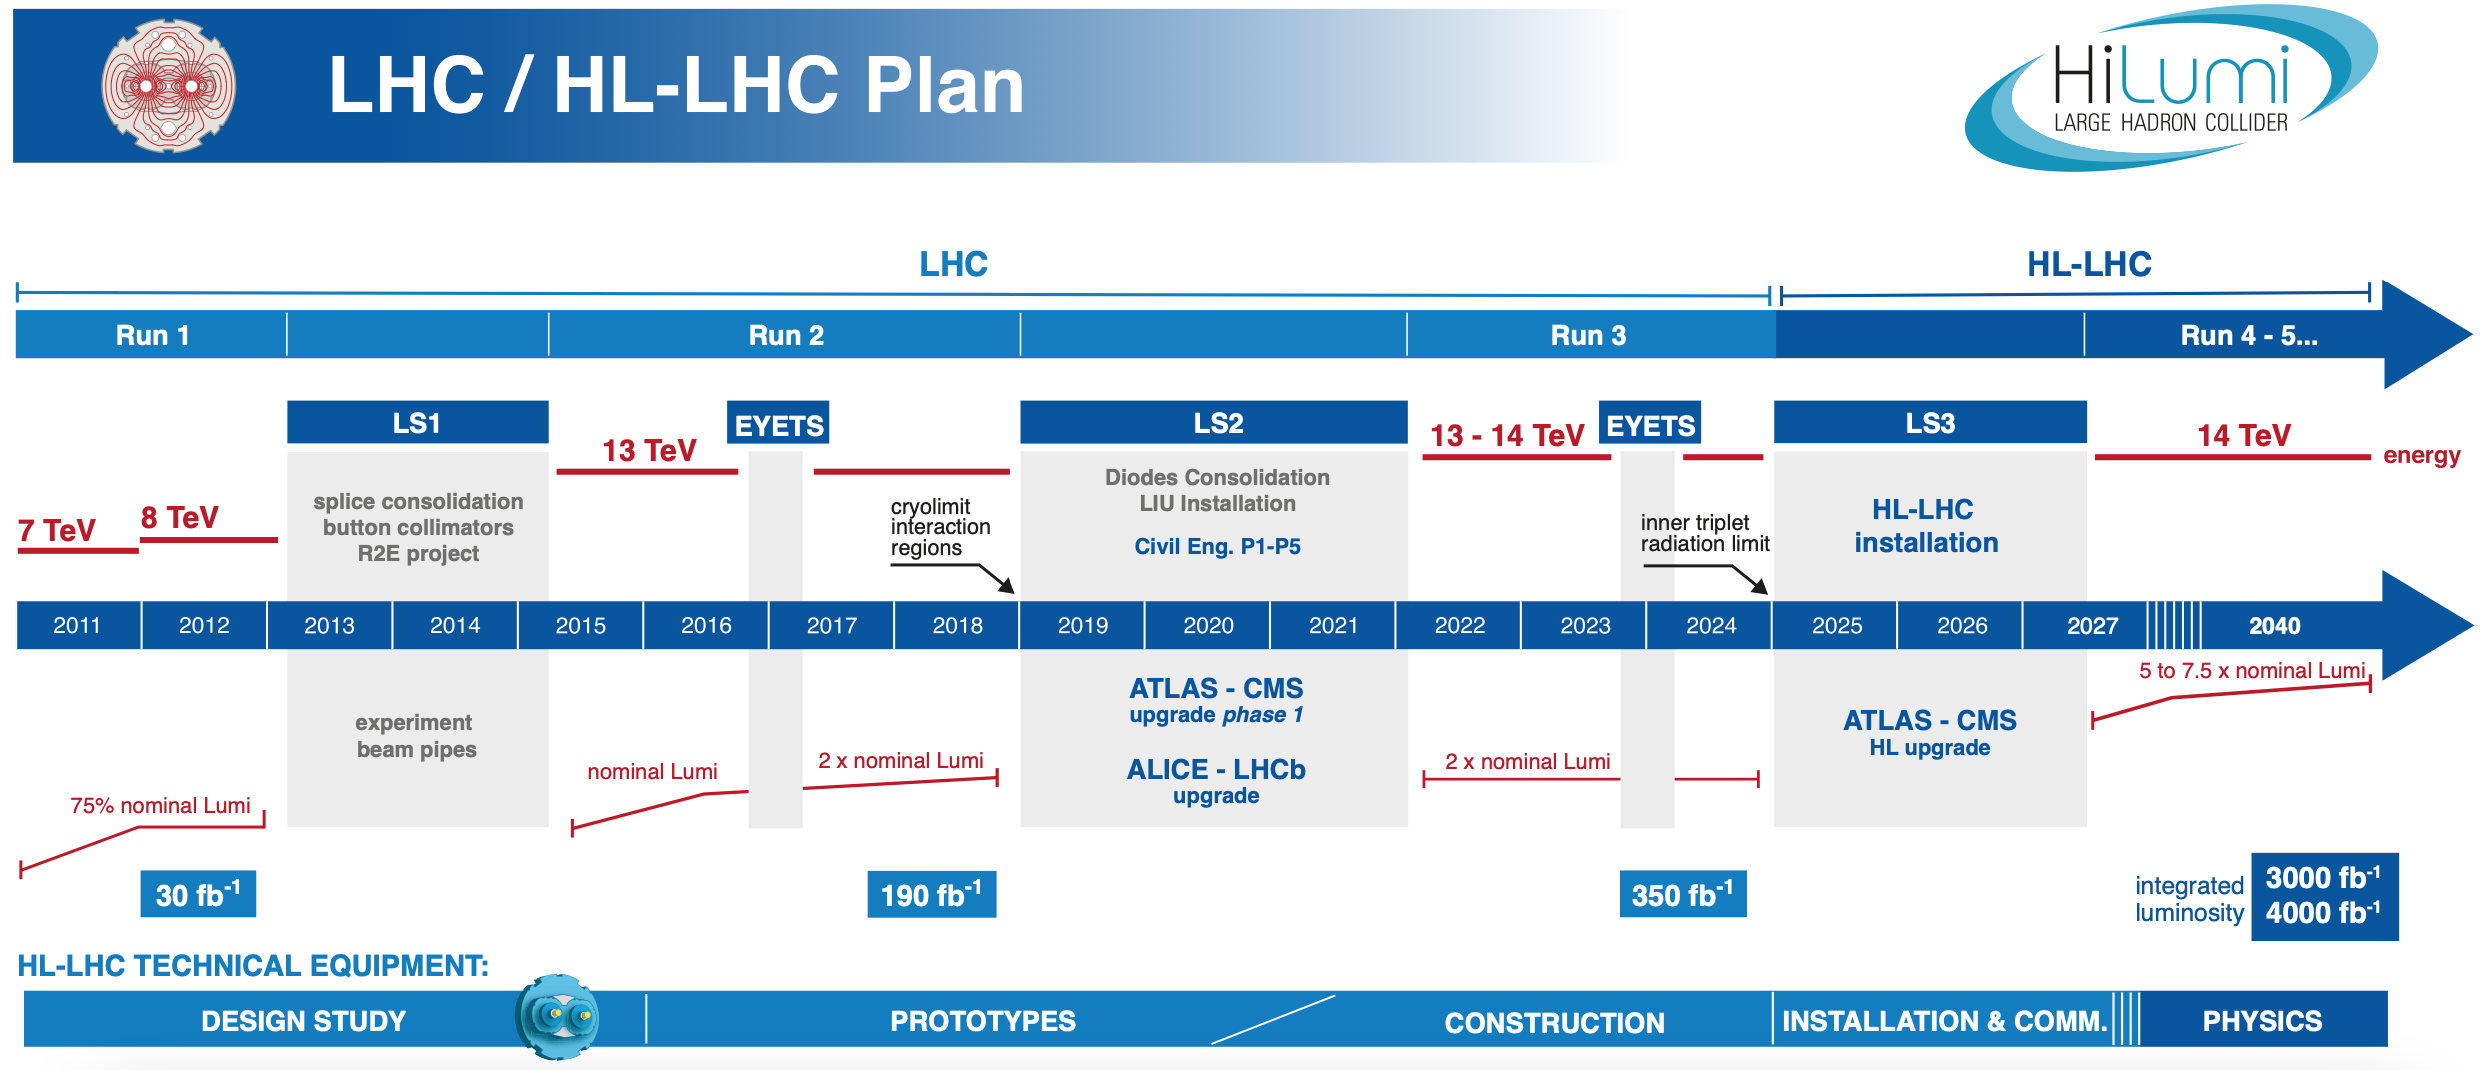
\includegraphics[width=\textwidth]{MSc_Thesis/fig/HLLHCplan.png}
	\vspace{2mm}
	\caption[A detailed schedule of LHC and HL-LHC showing the integrated luminosity and the beam energy corresponding to each period.]
	{A detailed schedule of LHC and HL-LHC showing the integrated luminosity and the beam energy corresponding to each period \cite{Apollinari:2284929}.}
	\label{HLLHCplan}
\end{figure}

The main scope of the HL-LHC is to increase the collision data which will allow physics searches to be more statistically abundant and be able to perform higher-precision measurements.

\subsection{The Accelerator Complex}

The accelerator tunnel of the LHC, which was previously used host LEP collider, has two parallel vacuum pipes where two counter-rotating beams are kept inside a magnetic field generated by superconducting niobium-titanium (NbTi) cables. The magnetic field generated to steer the beams are about 8 Tesla which is more than 100 000 times higher than the Earth2s magnetic field. This field is generated by  1232 dipole magnets each with a 14 metres of length and 35 tonnes of weight where 11 thousand Ampers of electric current flows. This acceleration system allow the beams to circulate with 7 TeV energy. The focusing of the beams in a narrow area is secured by 392 quadrupole magnets with 5 to 7 m lengths. In order to inject the beams in the collision points, special quadrupoles are positioned at each entrance to squeeze the beams in a narrower area. These superconducting magnets are cooled down to a temperature of 1.9 K by a cyrogenics cooling system supplied with 120 tonnes of Helium-4 fluid.

Before being injected into the LHC, the proton beams are pulled off from hydrogen gas and accelerated by a series of systems gradually increasing their energy, presented in \autoref{LHCacc}. Firstly, protons are accelerated to an energy of 50 MeV in the Linear Accelerator (LINAC2) then injected into the Proton Synchrotron Booster (PSB) where beams are re-accelerated to 1.4 GeV. These particles are sent to the Super Proton Synchrotron (SPS) to further accelerate them to 450 GeV energy. The final injection is made from the SPS to LHC's two beam pipes in the counter directions. The filling of the LHC by protons takes about 8 minutes, and 20 minutes for protons to be accelerated to 6.5 TeV of energy in bunches via Radio Frequency (RF) cavities operating. The injected beams circulate the LHC rings for many hours (12 hours) under normal operation. The bunches are spaced by 25 ns or 7.5 metres thus the bunch crossing rate is 40 MHz. Nominal number of protons per bunch is $12x10^{11}$ and the nominal number of bunches per beam is 2808 contributing to an inelastic collision event in the order of $10^9$ per second with about 20 collisions per bunch crossing.

\begin{figure}[ht]
	\centering
	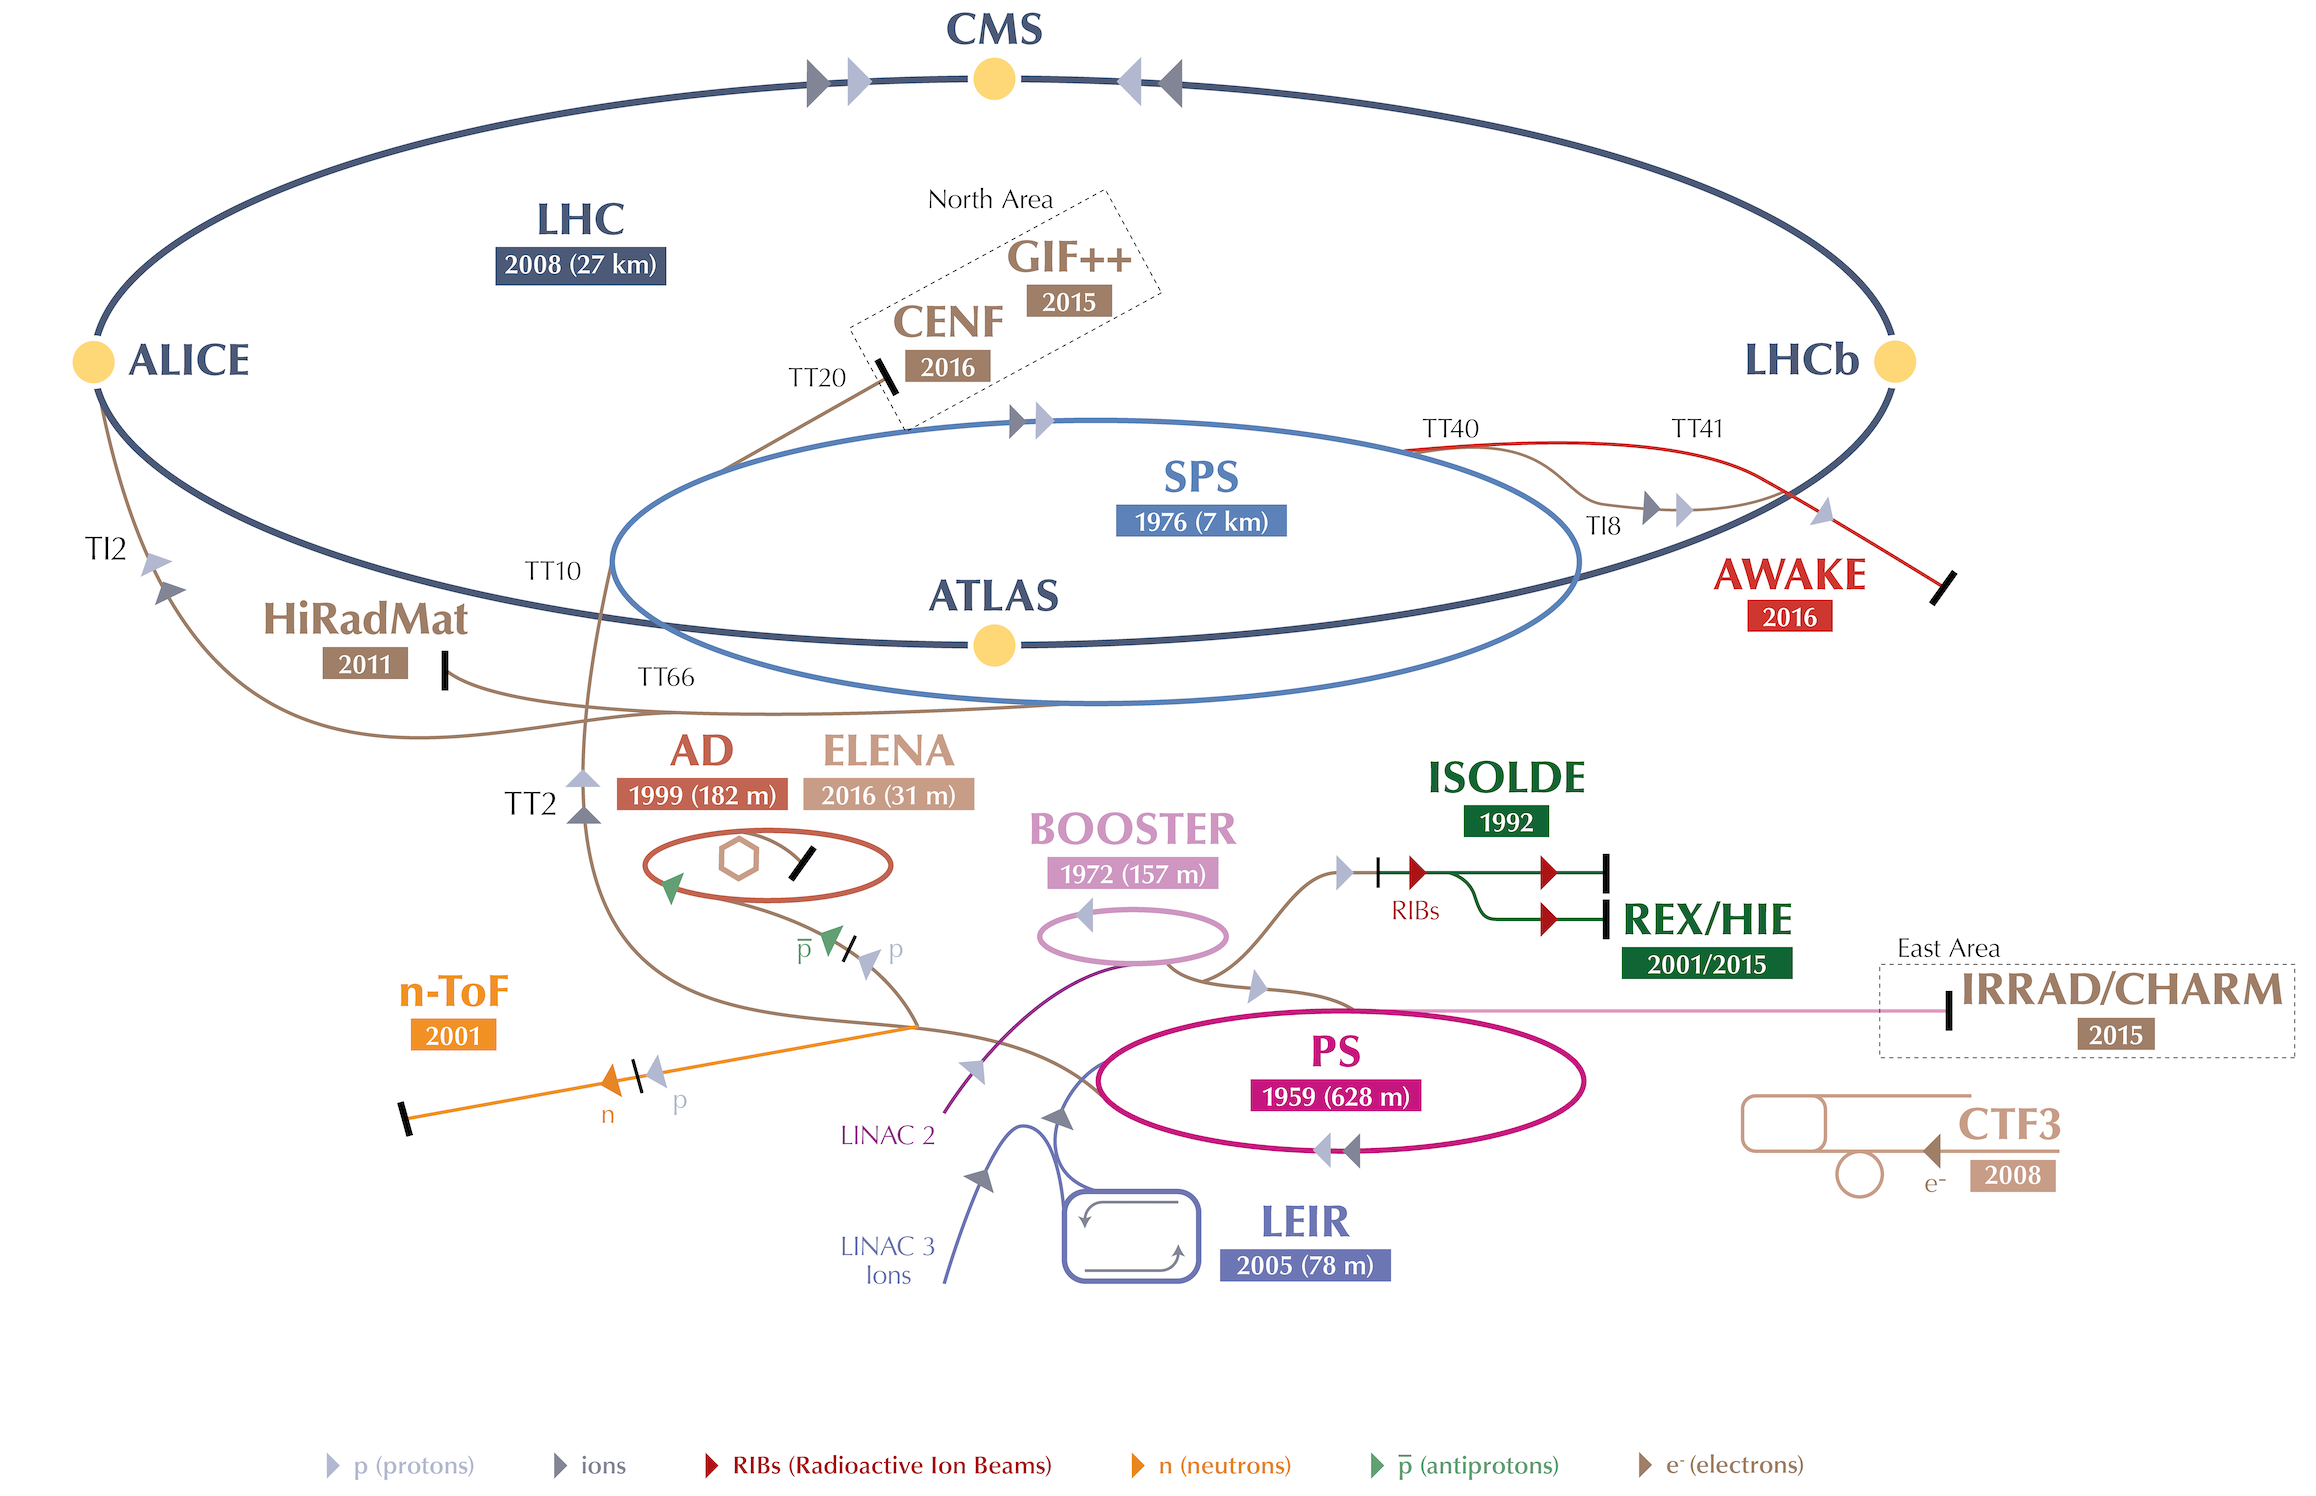
\includegraphics[width=\textwidth]{MSc_Thesis/fig/LHCacc.png}
	\vspace{2mm}
	\caption[The LHC accelerator complex. The acceleration of the protons start in the LINAC2 and ends in LHC through Booster, PS and SPS.]
	{The LHC accelerator complex. The acceleration of the protons start in the LINAC2 and ends in LHC through Booster, PS and SPS \cite{Mobs:2197559}.}
	\label{LHCacc}
\end{figure}

The accelerated beams of particles are collided inside one of the four detectors; ALICE, ATLAS, CMS and LHCb. The ATLAS and CMS Detectors are installed in opposite sides, at Point 1 and Point 5 of the LHC. These two detectors are designed as multi-purpose detectors that surround the collision points to detect any out-coming particle. They are described in detail in the references \cite{ATLAS2008, CMS2008}. ALICE Experiment is installed at Point 2 and its main purpose is to study heavy ion collisions and quark-gluon plasmas. Final of the four large experiments, LHCb, located at Point 8, is a forward one sided detector mainly aimed at measuring the charge conjugation and parity symmetry violation in Beauty baryons. The detailed description of the two detectors can be found in \cite{ALICE2008, LHCb2008}.

LHC host many other experiments; the LHCf \cite{LHCF2006} and TOTEM \cite{TOTEM2004} Experiments positioned at 100 meters away from the both sides of the ATLAS and CMS's collision points. These experiment study mainly the pp interactions and forward physics. Others are the MoEDAL\cite{moedal} Experiment which is dedicated to search for magnetic monopoles at the same experimental cavern with LHCb detector, and the FASER Experiment searching for lighter particles and studying neutrinos situated 480 metres away from the ATLAS's collision point.

\subsection{Design and specifications}

The \textbf{\emph{collision energy}} of the particles inside the detectors is one of the most important parameters at the LHC and is simply the sum of the energy of two colliding beams. When these collisions happen, independent types of interactions may happen between protons. The \textbf{\emph{soft interactions}} signify a small amount of transferred momentum which means the interacting protons barely came close to each other and escapes without decaying at all. The \textbf{\emph{hard interactions}} on the other hand, signify a high transferred momentum which causes the proton to decay. When two protons collide, a fraction of the energy ($s\prime$) contributes to the interaction since it is actually the partons of the protons that participate in the collision proportional to the fraction of energies ($x_1,\; x_2$) of each parton.
\be
\sqrt{s\prime} = \sqrt{x_1 x_2 s}
\ee
Another important parameter is the \textbf{\emph{instantaneous luminosity}} for the LHC apparatus. It is a description of the number of collisions per time and cross section. It is given by the following formula,
\be
L = \frac{N_b^2 n_b f_{rev} \gamma}{4 \pi \epsilon_n \beta}F \; ,
\ee
where $N_b$ is the number of particles in each bunches of $n_b$ bunches circulating in the accelerator ring with $f_{rev}$ frequency. The parameters $\gamma$, $\epsilon_n$, $\beta$ and the factor $F$ denotes the relativistic Lorentz factor; emittence and focal length describing the shape and focus of the beam, and geometrical reduction which depends on the angle between two beams, respectively. The luminosity lifetime $\tau$ on the other hand shows how luminosity decreases with time,
\be
L = L_0 e^{-t/\tau} \; ,
\ee
where $L_0$ is the peak luminosity at time zero.

The integrated luminosity, which is another important parameter, is given by $L = \int L dt$ and takes part in the total amount of collisions over time.
\be
N = L x \sigma
\ee
is the number of events produced for a particular physics process with the cross section $\sigma$. Thus, in order for a rare process to be observed in the detectors, maximising the luminosity is essential. In \autoref{SMcrosssections}, the cross sections as a function of $\sqrt{s}$ is shown. It is obvious that the Higgs processes are several orders of magnitude lower in production cross section than the dominant processes, however since the cross section increases with the increasing centre-pf-mass energy, it is necessary to increase also luminosity and $\sqrt{s}$ in order to achieve higher event rates. The integrated luminosity delivered to the CMS experiment since 2010 is shown in \autoref{CMSlumi}.
\begin{figure}[ht]
	\centering
	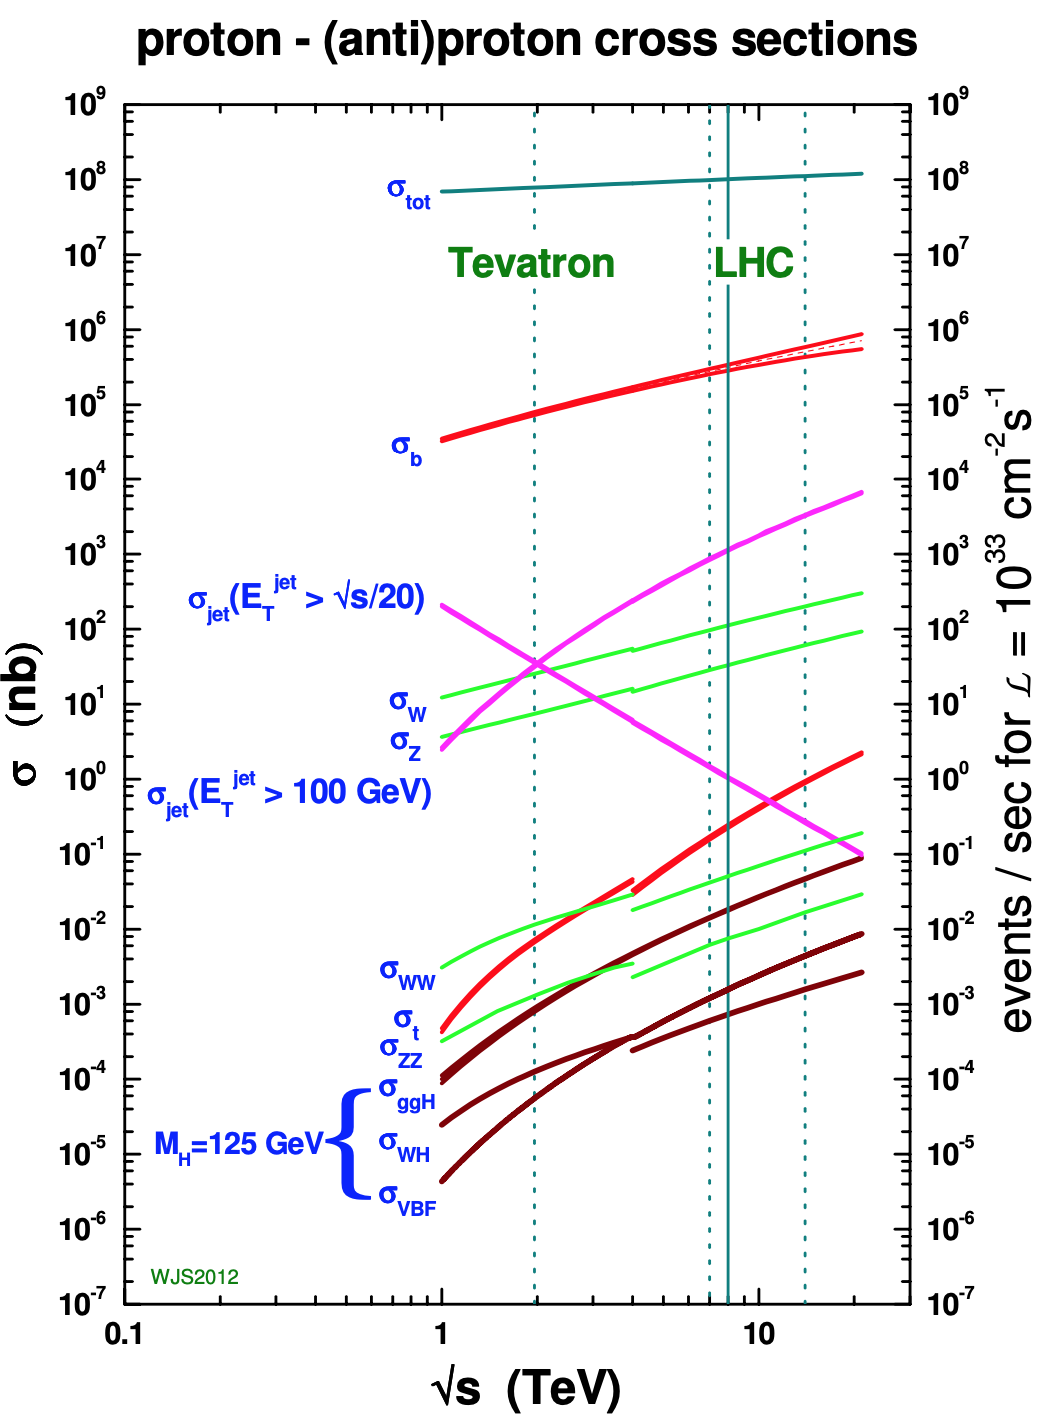
\includegraphics[scale=0.5]{MSc_Thesis/fig/stirling.png}
	\vspace{2mm}
	\caption[Cross sections of Standard Model processes as function of collider energy at pp collisions.]
	{Cross sections of Standard Model processes as function of collider energy at pp collisions\cite{stirling}.}
	\label{SMcrosssections}
\end{figure}

The large instantaneous luminosity of the LHC causes a disadvantage. Multiple pp collisions happen at each bunch crossing and many primary vertices are superimposed. Most of these parton interactions have relatively small centre-of-mass energy, hence they are not of much interest for the experiment, which is often called \textbf{\emph{in-time pileup (PU)}} interactions. Therefore, the detector needs to resolve these pileup interactions from the hard collisions. Besides, since the collisions take place at the heart of the CMS detector, it is inevitable that new particles reach the detector before the products of the previous bunch crossing escapes the detector. This type of pile up is called \textbf{\emph{out-of-time pileup}} interactions. In order to overcome these demanding conditions, highly granular and fast-response detectors are needed. Moreover, the detector needs to be resistant to radiation as well as be precise in energy measurements. The Compact Muon Solenoid, an appropriate detector designed to overcome these challenges, is explained in the next section.

\begin{figure}[ht]
	\centering
	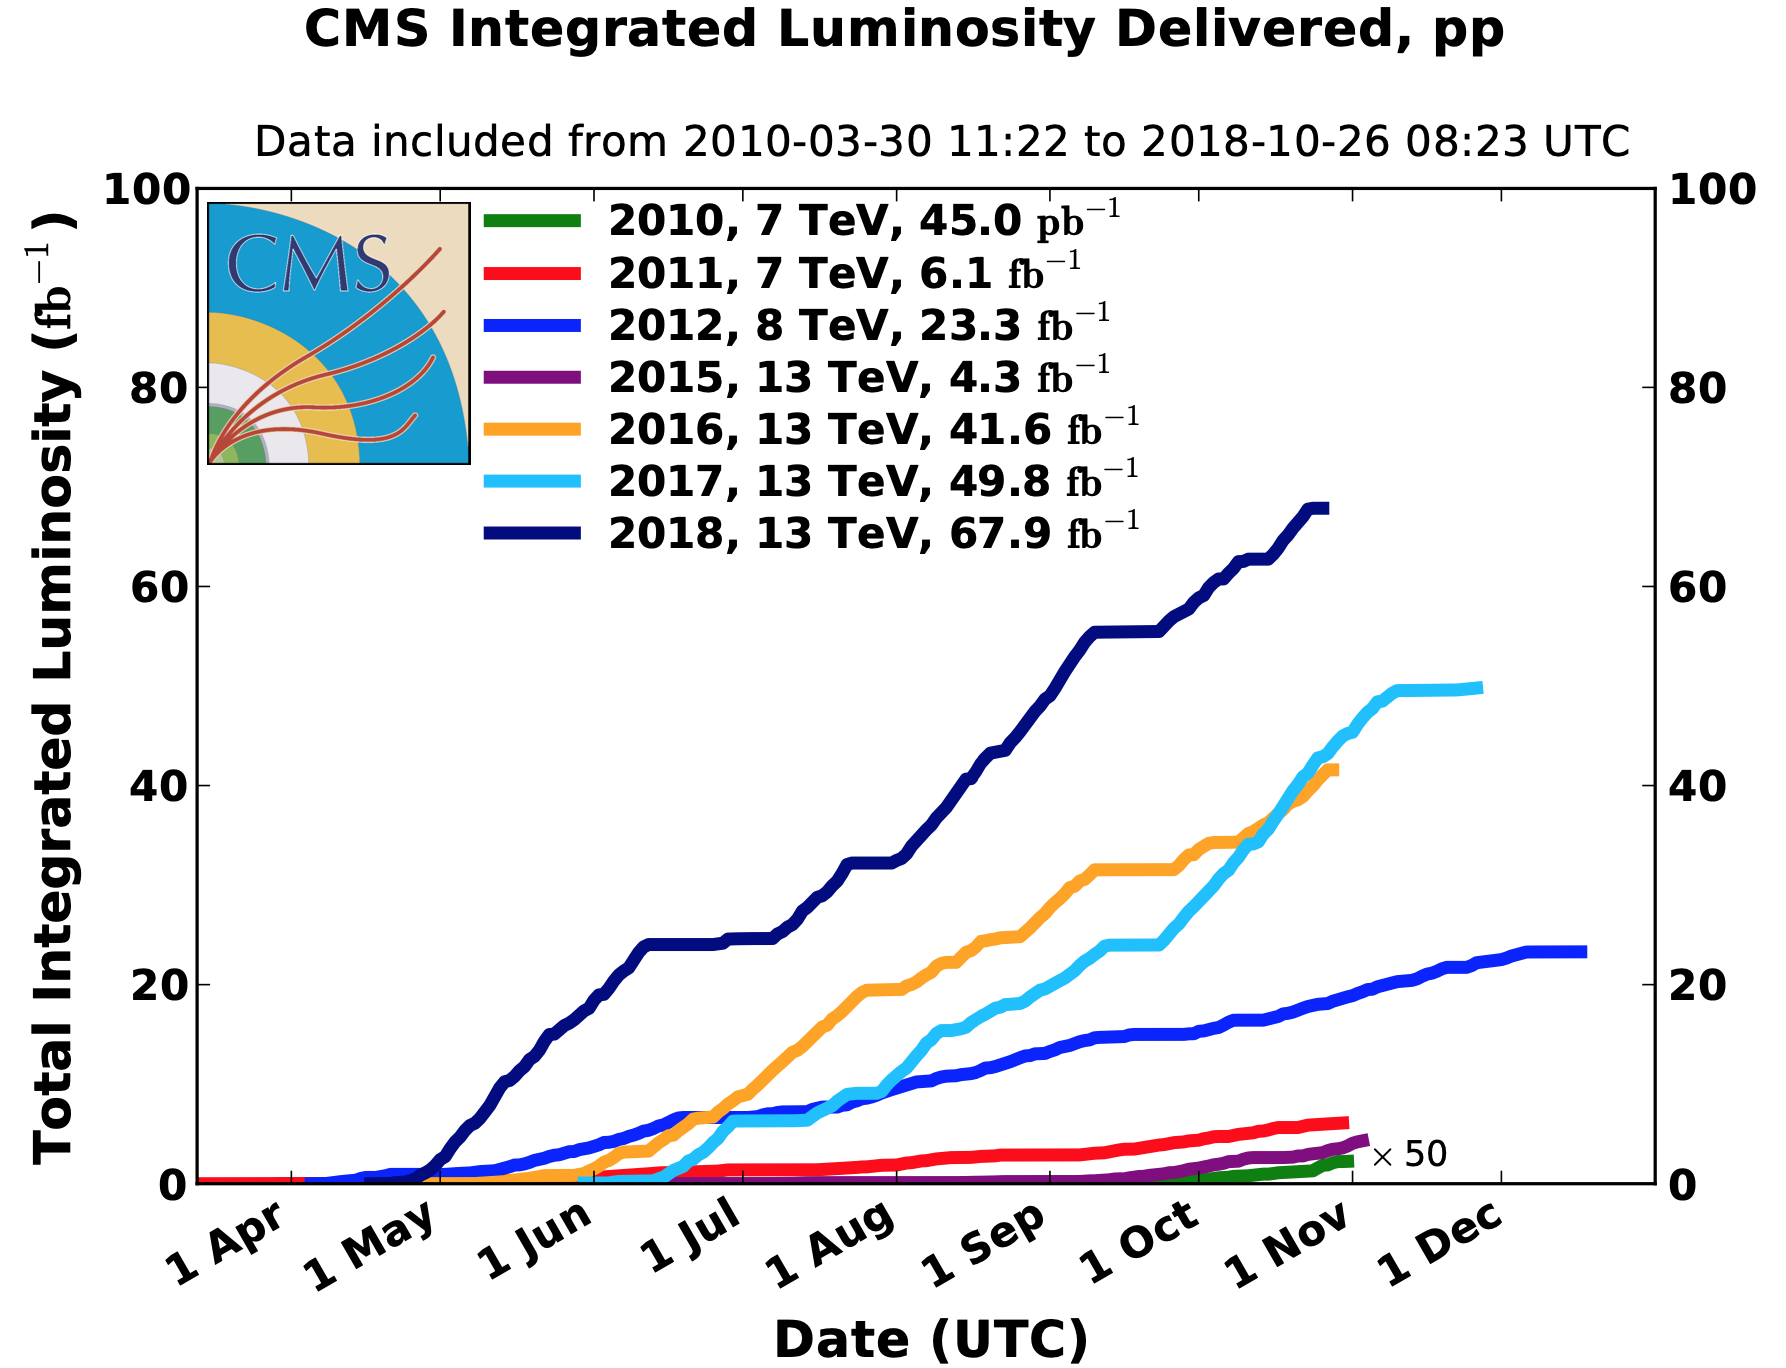
\includegraphics[scale=0.4]{MSc_Thesis/fig/CMSlumi.png}
	\vspace{2mm}
	\caption[Total integrated luminosity delivered by the LHC to the CMS detector for pp collisions at Run I-II.]
	{Total integrated luminosity delivered by the LHC to the CMS detector for pp collisions at Run I-II \cite{CMSlumi}.}
	\label{CMSlumi}
\end{figure}











